\chapter{Prevádzka a bezpečnosť sietí}
\phantomsection
%TODO MOZNO NIECO O PREVADZKE SIETI + BEZPECNOSTNY ASPEKT
Prevádzka sieťových zariadení je proces nielen o monitorovaní incidentov, zabezpečovaní konzistencie a konvergencie siete, ale aj o aktualizáciách softvéru a hardvéru, aplikovaní bezpečnostných zásad a politík. Táto kapitola preto opisuje jednotlivé aspekty s ktorými sa pri prevádzke siete môžeme stretnúť.

\section{Sieťové prvky}
Medzi základné stavebné piliere sietí, bez ktorých nie je možná komunikácia koncových staníc patria smerovače (router) a prepínače (switch). Mimo týchto dvoch základných zariadení sa v \zkratka{zkLAN} sieťach často vyskytujú prístupové body (access point), firewally, sieťové mosty (bridge) a v dnes už ojedinelých prípadoch ešte aj rozbočovače (hub). V súčasnosti však jedno zariadenie môže kombinovať funkcie zariadení, ktoré majú podľa modelov TCP/IP alebo ISO/OSI na starosti inú vrstvu modelu. Preto sa dnes hlavne z finančných dôvodov používajú takzvané L3 prepínače, ktoré s určitými obmedzeniami vedia nahradiť nákladné smerovače. Taktiež smerovače ako aj L3 prepínače umožňujú filtrovanie paketov, takže vedia čiastočne zastať aj základné funkcie firewallu. Značky najpoužívanejších sieťových zariadení su vyobrazené na obrázku \ref{net-devices} a budú používané v nasledujúcich kapitolách.

\begin{figure}[H]
	\begin{center}
		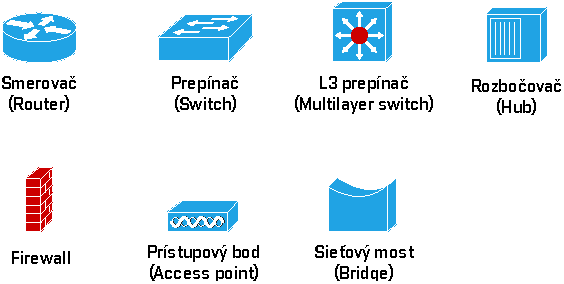
\includegraphics[scale=0.4]{obrazky/net_devices.pdf}
	\end{center}
	\vspace{-5em}
	\caption[Typy sieťových zariadení v lokálnych sieťach]{Typy sieťových zariadení v lokálnych sieťach}
	\label{net-devices}
\end{figure} 

\section{Hierarchický model sietí}
%TODO EDGE
S postupným nárastom sieťových zariadení a komplexnosti siete dochádza v sieťach bez hierarchie k mnohým problémom ako veľké broadcast domény, vysoká cena za port, vysoké zaťaženia zariadení, neprítomnosť redundancie. Preto sa zaviedol hierarchický model siete, ktorý rieši problémy veľkosti a rozsahu broadcast a kolíznych domén, umožňuje efektívne prideľovanie \zkratka{zkIP} adries a oddeľuje zariadenia pracujúce na jednotlivých vrstvách ISO/OSI.  
\\\\
\noindent
Siete sú spravidla delené do 3 vrstiev s definovanými funkciami \cite{Lammle2013}:
\begin{itemize}
	\item Core\,--\,tvorí vysokorýchlostnú chrbticu siete, agreguje dáta z distribučnej vrstvy a mala by byť redundantná. Nároky na rýchlosť portov a výkon zariadenia sú obzvlášť vysoké, a preto sa využívajú prevažne smerovače, ale taktiež ako v distribučnej vrstve dnes už aj L3 prepínače.
	\item Distribučná (Distribution)\,--\,agreguje dáta z prístupovej vrstvy, vytvára a oddeľuje broadcast domény, riadi smerovanie medzi \zkratka{zkVLAN} a  filtrovanie paketov. Táto vrstva kvôli zabezpečeniu dostupnosti využíva agregovanie  a redundanciu liniek. Typicky sa skladá zo smerovačov, no v dnešnej dobe hlavne z L3 prepínačov, keďže tie nie sú finančne také náročné. 
	\item Prístupová (Access)\,--\,vstupný bod do siete, ktorý riadi prístup a politiku pre koncové zariadenia, segmentuje sieť, vytvára a separuje kolízne domény. V neposlednej rade zariaďujú prístup k distribučnej vrstve. Je tvorená zariadeniami ako prepínač, rozbočovač alebo prístupový bod.
\end{itemize} 

\begin{figure}[H]
	\begin{center}
		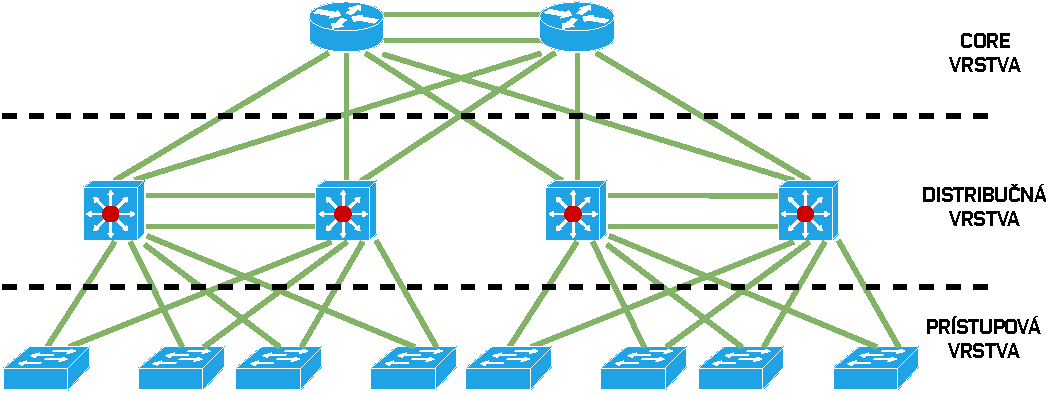
\includegraphics[scale=0.58]{obrazky/hierarchy_network.pdf}
	\end{center}
	\vspace{-11em}
	\caption[Hierarchické rozdelenie siete na vrstvy]{Hierarchické rozdelenie siete na vrstvy}
	\label{net-devices}
\end{figure} 

\noindent
\vspace{2em}
V menších sieťach prevažne malých firiem sa využíva zlučovanie vrstiev nazývaných ako collapsed core, ktoré zlučujú distribučnú a core vrstvu, prípadne zlučujú všetky tri vrstvy dokopy. 

Cieľom hierarchického modelu a dobre navrhnutej siete je dosiahnutie nasledujúcich vlastností:

\begin{itemize}
	\item Škálovateľnosť\,--\,jednoduché a bezproblémové pridanie zariadenia pri raste a rozširovaní siete.
	\item Redundancia\,--\,zabezpečenie vysokej dostupnosti viacnásobnými linkami medzi zariadeniami a zálohovanie samotných zariadení ich redundanciou.
	\item Výkonnosť\,--\,agregovanie liniek a výber dostatočne výkonných zariadení
	\item Bezpečnosť\,--\,zabezpečenie siete na viacerých úrovniach ako napríklad portoch, oddelením segmentov pomocou VLAN, riadením prístupu, šifrovaním a pod.
	\item Manažovateľnosť\,--\,vytvorenie šablón, definovaných štandardov a pravidiel na zaistenie konzistentnosti konfigurácií zariadení na jednoduchšie odhaľovanie chýb. 
	\item Udržovateľnosť\,--\,schopnosť systému prechádzať zmenami komponentov, služieb a vlastností.
\end{itemize}



\section{Úrovne sieťových prvkov}
Sieťové prvky sú zodpovedné nielen za preposielanie dát medzi koncovými stanicami, ale aj za mnohé riadiace dáta medzi sebou, bez ktorých by sieť nebola funkčná. Preto sa jednotlivé protokoly a služby rozdeľujú troch rovín alebo úrovní, a to management, control a data plane. Tieto pojmy sa využívajú vo väčšej miere v softvérovo definovaných sieťach, no sú platné aj v klasickej koncepcii.
 
Úroveň management plane je zodpovedná za konfiguráciu zariadení a riadenie prístupu ku konfiguráciám. Typickými príkladmi protokolov pracujúcich na tejto úrovni sú \zkratka{zkSNMP}, \zkratka{zkAAA}, Syslog, \zkratka{zkSSH} a mnohé ďalšie \cite{Singh2018}. Druhá úroveň, control plane má na starosti prevažne smerovanie, teda kadiaľ budú pakety smerované a prenáša riadiace a signalizačné informácie pre protokoly ako napríklad, \zkratka{zkOSPF}, Spanning tree, \zk{zkFHRP} \cite{Singh2018}. Poslednou úrovňou je data plane nazývaná často aj forwarding plane, ktorá prepína pakety na daný port na základe rozhodnutie z control plane. Táto časť sieťových prvkov musí byť veľmi rýchla, aby zaistila nízku odozvu a dostatočne vysoké prenosové rýchlosti. Nižšie uvedený obrázok \ref{sdn-planes} reflektuje tok dát z jednej úrovne do druhej a tiež medzi dvoma susednými zariadeniami. Úroveň management plane zodpovedná za konfiguráciu zariadenia a nastavuje úroveň control plane, v tomto prípade smerovanie z zariadení. Po výmene informácií so susednými smerovačmi sa vytvoria príslušné tabuľky a nakoniec smerovacia tabuľka, ktorá sa využíva pri rozhodovaní prepínania paketov v úrovni data plane.

\begin{figure}[H]
	\begin{center}
		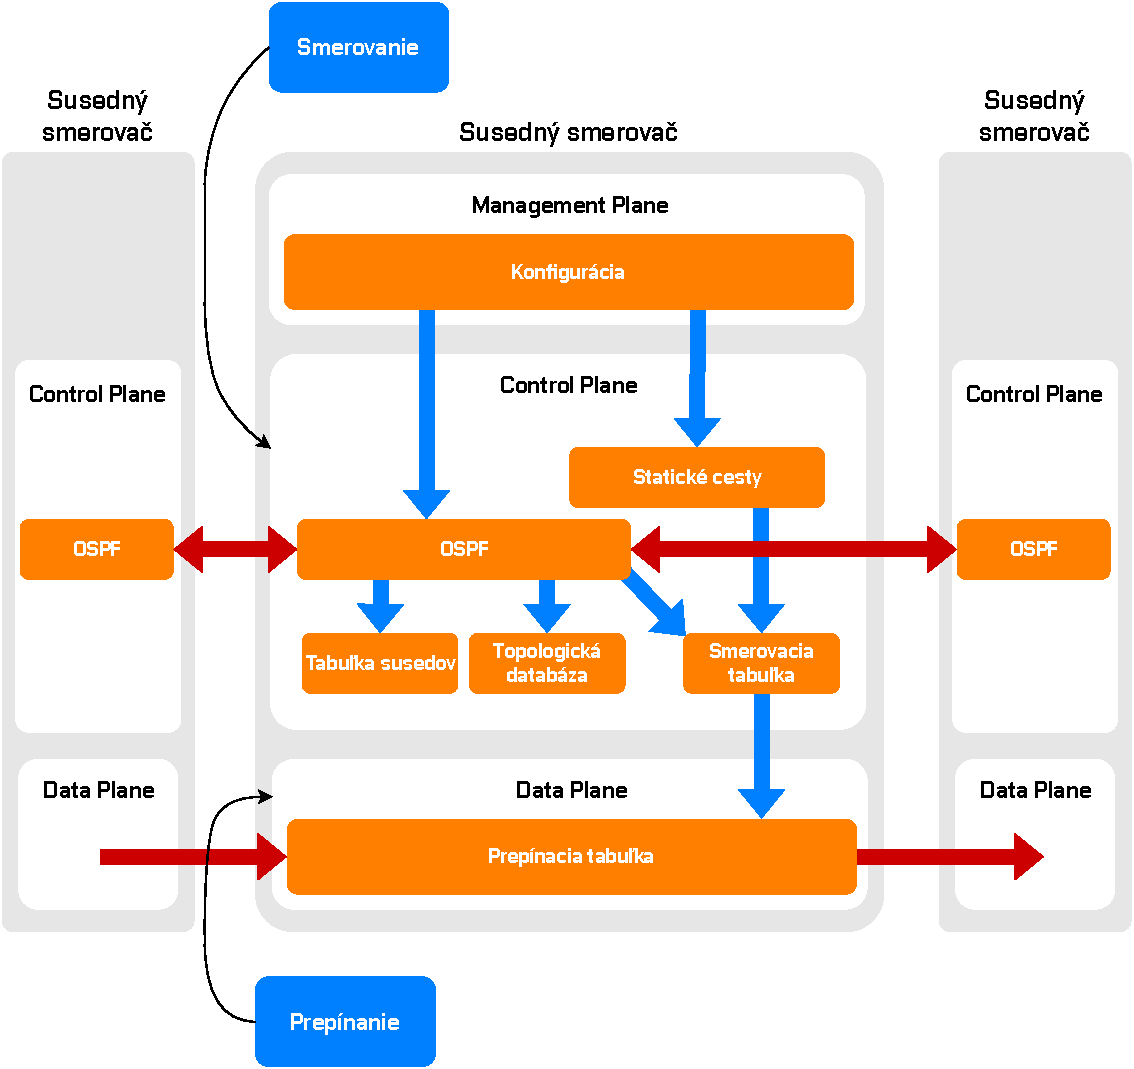
\includegraphics[scale=0.6]{obrazky/SDN_planes.pdf}
	\end{center}
	\caption[Rozdelenie úrovní v smerovači, tok informácií v jeho vnútri a medzi susednými smerovačmi]{Rozdelenie úrovní v smerovači, tok informácií v jeho vnútri a medzi susednými smerovačmi \cite{Pepelnjak2013}}
	\label{sdn-planes}
\end{figure} 


%TODO 3 za tried source interfaces


\section{Riadenie a zneužitie prístup}
AAA, username, accounts, enable psswd, ssh, ACL(data plane, je to data plane?) 92, 111, 112, bannery plus logovanie neuspesnych pristupov

\section{Smerovacie protokoly}
autentizacia, passive, ip source routing, urpf


\section{Identifikácia zariadení, pravidiel a nastavení}
host,domainname, acl remark, int description, vlan description

\section{Šifrovanie hesiel}

\section{Logovanie}
syslog, snmp nastavenie oboch, plus co logovat, teda accouting a logovanie deny pravidiel, 93

\section{Synchronizácia času}
ntp + amplifikacne utoky

\section{Záloha a zabezpečenie konfigurácií}
archive, tftp, scp, delete protection, logovanie zmien, mozno netreba, ak je AAA accounting
\section{Správanie pri vysokom zaťažení}
68-71, storm control
\section{Monitorovanie výkonu siete}
SPAN NETFLOW
\section{Problémy vrstvy L2}
access, max, hopping, double tagging, blackhole, default access a trunk, dtp, spanning tree, dot1x, vtp
\section{First Hop Security}
130 - 138 140 144-148 aj mac spoof a mac floof, teda spanning tree prikazy!!!
http://isp-servis.com/?p=191
\section{First Hop Redundancy Protocols}

\section{Tunely}
\section{Mapovanie siete a objavovanie zariadení}
proxy arp, 88-91, lldp, cdp, 139
\section{Nepoužívané a nebezpečné služby}
\section{Ostatné}
source interfaces
loopback
shutdown 